\chapter{数据认证方案优化}
本章讨论对无线传感网多节点联合数据认证机制进行优化,利用多种方案提升数据认证机制的检测效率,降低节点能量消耗。
4.1节介绍无线传感网节点失效问题,提出了多路径抗节点失效的机制。
4.2节设计动态步长的多节点联合数据认证机制。
\section{多路径抗节点失效机制}
由于无线传感网部署的环境恶劣,且容易受到攻击,使得节点的稳定性很难保证,整个网络的拓扑结构很容易发生变化。在3.3节中,我们讨论了在拓扑结构变化频率不大的情况下,通过传感器网络自身的维护机制,维护路径节点的上下行相关关系,适应无线传感网拓扑结构的变化。但是在节点失效或者被攻击比较频繁时,无线传感器网络结构变化很快,而原有的维护方案是通过重建路径来完成的,因而通信开销较大,造成大量节点能量损耗。

为了适应节点失效较多,传感网拓扑结构变化较大的情况,我们提出了多路径抗节点失效的方案。通过在初始化阶段预定义若干条不相交路径,对每个节点失效的情况预定义编织路径。但在一个传输阶段,只有一条路径被使用,并进行数据认证。当路径受到攻击,或者节点失效时,使用备用的不相交路径或者编织路径。

在多路径抗节点失效方案中,我们使用了单向hash链来分配密钥,提升了网络的安全性能,并节省了节点存储密钥的开销。每个节点使用单向hash函数从它的上行相关节点的密钥生成密钥,具体的密钥分配方案将在第五章进行详细描述。
\subsection{设计实现}
在多路径抗节点失效机制中,节点上下行相关关系不是研究重点,不再详细介绍,沿用第三章中多跳长路径多节点联合数据认证的方案。我们在多路径抗节点失效机制中,使用了单向hash链来分配密钥,能更好地保证认证机制的安全性,降低节点保存密钥的存储开销。我们的路径抗节点失效机制包括了初始化和密钥分配、数据报文发送、路径中过滤、基站认证、路径选择五个阶段。
\subsubsection{初始化和密钥分配}
传感器节点被部署到目标监测区域之后,基站会给每个节点生成一个共享密钥,这是每个节点与基站之间的共享密钥$AK_{si}$。然后每个簇通过预定的选举机制选举一个簇头节点,BS通过广播路由请求完成传感器网络的路由发现。

在多节点联合数据认证方案中,我们使用HELLO报文和ACK报文来完成路径发现和上下行相关关系的建立,在簇与BS之间建立一条多跳长路径。在多路径抗节点失效方案中,我们在初始化建立多条不相交长路径以及多条编织路径。虽然有多条路径,在我们的方案中,一次传输过程只会使用一条主路径,其他路径作为网络被攻击时的备选路径。

\begin{figure}[htbp]
  \centering
  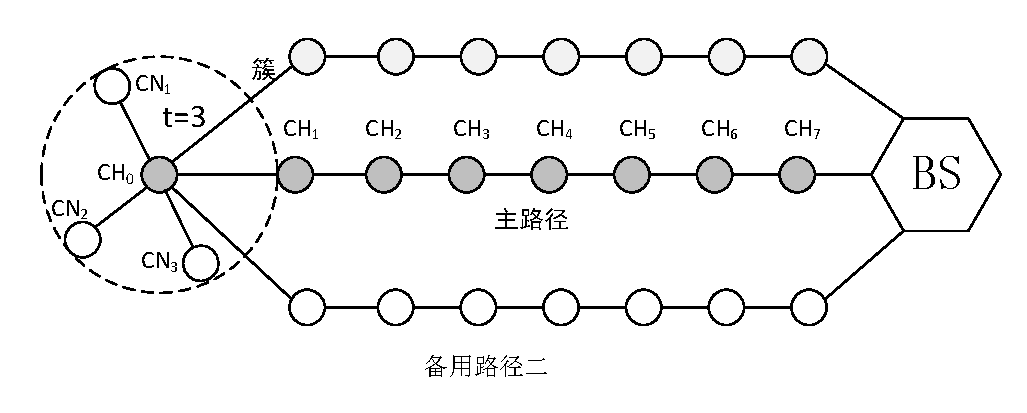
\includegraphics[width=5in]{IHAA1}
  \caption{多路径抗节点失效机制中的不相交路径}
  \label{fig:IHAA1}
\end{figure}
如图~\ref{fig:IHAA1}所示,簇与BS之间建立了3条不相交路径。不相交路径通过以下步骤建立:
\begin{compactitem}
  \item 建立一条簇头与BS之间的主路径。
  \item 建立一条与主路径不相交的,且跳数最短的路径,作为备用路径一。
  \item 建立一条与主路径以及备用路径一不相交的,且跳数最短的路径,作为备用路径二。
\end{compactitem}

\begin{figure}[htbp]
  \centering
  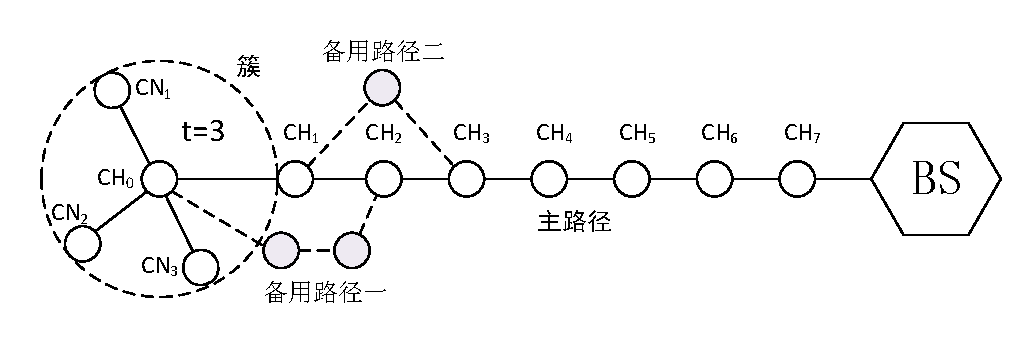
\includegraphics[width=5in]{IHAA2}
  \caption{多路径抗节点失效机制中的编织路径}
  \label{fig:IHAA2}
\end{figure}
如图~\ref{fig:IHAA2}所示,路径上的节点完成备用编织路径的建立。编织路径通过以下步骤建立:
\begin{compactitem}
  \item 建立一条簇头与BS之间的主路径。
  \item 对主路径上的每个节点,寻找不包括该节点的簇与BS之间的最短路径。在图~\ref{fig:IHAA2} 中,第一条编织路径就是不包括节点$CH_1$,从节点$CH_0$到节点$CH_2$之间的编织路径。相似的,第二条编织路径是不包括节点$CH_2$的从节点$CH_1$到节点$CH_3$的编织路径。
\end{compactitem}

\begin{figure}[htbp]
  \centering
  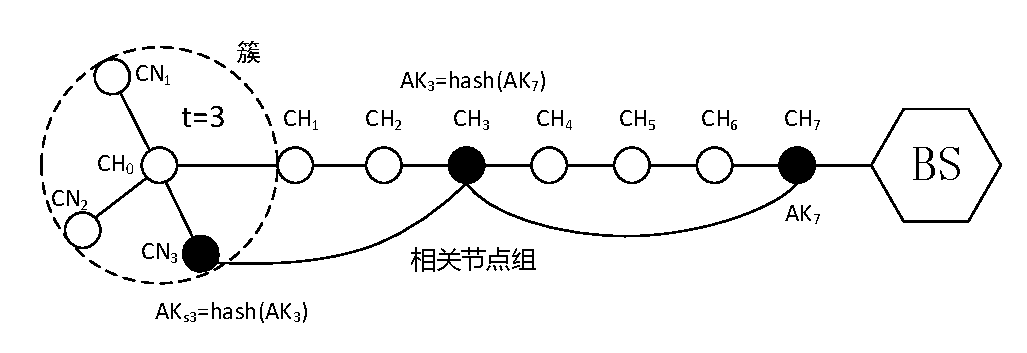
\includegraphics[width=5in]{IHAA3}
  \caption{多路径抗节点失效机制的密钥分配}
  \label{fig:IHAA3}
\end{figure}
在我们的多路径抗节点失效方案中,我们使用了单向hash链来进行密钥分配,如图~\ref{fig:IHAA3}所示。BS给每个上下行相关节点组生成一个$AK$,下行节点使用单向hash函数$H$从上行节点的密钥得到自己的密钥。图~\ref{fig:IHAA3}中所示,节点组\{$CN_3$,$CH_3$,$CH_7$\},距离BS最近的节点$CH_7$从BS获取BS生成的密钥$AK_7$,它的下行节点$CH_3$通过单向hash函数获取密钥$AK_3=H(AK_7)$。类似的,节点$CN_3$获取密钥$AK_{s3}=H(AK_3)$。通过这样的密钥分配,每个节点存储密钥的空间开销变小了,同时节点被攻击时丢失的密钥信息变少了。
\subsubsection{数据报文发送}
同多节点联合数据认证一样,簇节点监测到事件E以后,必须要$t+1$个节点都发出报文才能确认监测到的事件,如果没有至少$t+1$个节点的报文,则认为是无效事件。
簇节点MAC压缩后记作$XMAC(E)$:
\begin{equation}\label{XMAC}
\begin{split}
  XMAC(E)
  &=MAC(AK_{s1},E)\oplus MAC(AK_{s2},E)\oplus MAC(AK_{s3},E)\oplus MAC(AK_{s0},E)
\end{split}
\end{equation}
在多路径抗节点失效方案中,我们使用簇序号$C_i$来标记簇信息,代替原方案中的簇ID集,减小了传输开销。在簇头节点$CH_0$生成的报文R可以记作:
\begin{equation}\label{report1}
\begin{split}
  R=
  & E,C_i,h_0,XMAC(E),\{MAC(AK_{s1},E),\\
  & MAC(AK_{s2},E),MAC(AK_{s3},E),MAC(AK_0,E)\}
\end{split}
\end{equation}
\subsubsection{路径中过滤}
当节点$CH_i$从下行节点收到报文R以后,首先用相邻节点共享密钥对进行认证。然后使用其上下行相关节点的共享密钥对E计算MAC,并更新报文R。对于图~\ref{fig:IHAA3}中的节点$CH_3$,收到来自$CH_2$ 的报文后,首先使用单向hash函数计算得出其下行相关节点的密钥$AK_{s3}=H(AK_3)$。用$AK_{s3}$对事件$E$计算消息认证码$MAC(AK_{s3},E)$,与报文R中的第
$(h_0 - h_i)-((h_0 - h_i)/(t+1))\ast (t+1)=3$ 个相关节点MAC,也就是$MAC(AK_{s3},E)$进行比较,如果不同则丢弃报文R;如果相同则使用密钥$AK_3$ 对事件E计算消息认证码$MAC(AK_3,E)$,并替代原报文R中的$MAC(AK_{s3},E)$,将其转发给下一节点$CH_4$,更新后发送的报文R 为:
\begin{equation}\label{report2}
\begin{split}
  R=
  & E,C_i,h_0,XMAC(E),\{MAC(AK_1,E),\\
  & MAC(AK_2,E),MAC(AK_3,E),MAC(AK_0,E)\}
\end{split}
\end{equation}

\subsubsection{基站认证}
当BS收到报文R后,首先获取报文中的簇序号$C_i$,使用BS与簇$C_i$的节点ID列表中$t+1$个簇节点之间的共享密钥计算MAC,并用XOR 运算计算这$t+1$ 个MAC 的值,与报文R中的XMAC比较,如果不同,则丢弃报文。如果相同,则对事件E作出响应。
\subsubsection{路径选择}
当路径中节点受到攻击时,BS会收集到相应的信息,通过妥协节点检测技术\upcite{c4:mathews2007detecting},BS能确定哪些路径被攻击,妥协节点检测技术不是本文的重点,而是专注于妥协节点检测技术在数据认证中的应用。当BS确定了受攻击的路径以后,切换到未被攻击的备用路径。

同多节点联合数据认证机制中的节点关系维护相比,我们的多路径抗节点失效是通过预先定义备用路径,是一个应对节点攻击的前瞻性安全机制。而多节点联合数据认证机制中的节点维护是一种即时修复的方法,在节点失效或被攻击频率较高时,会造成传感器网络的传输路径不稳定,受攻击的影响更严重,还会造成大量的节点能量消耗。
\subsection{安全性能分析}






\section{动态步长多节点联合数据认证}
在无线传感网的多跳长路径传输中应用我们的多节点联合数据认证机制,能有效保证数据的安全传输,但是数据报文中附带了大量的MAC信息,加重了传感器节点的能量消耗。因此我们提出了一个动态步长的多节点联合数据认证,在传感器网络节点受攻击影响较小的时候,压缩所传输的报文,降低节点能量消耗。
\subsection{动态步长多节点联合数据认证机制设计}
动态步长多节点联合数据认证是在多节点联合数据认证的基础上,对其进行改进,使得通信开销得到优化。
在4.1节中,我们讨论了在传感网拓扑结构变化较大时,使用多路径抗节点失效的机制来保证传感网传输稳定性。对于一条簇到BS之间的传输路径,如果路径比较稳定,则可以通过压缩数据报文的方式来降低传输开销。在我们提出的动态步长多节点联合数据认证机制中,是通过动态调整多节点联合认证中的节点组间隔步长来实现的。

在多节点联合数据认证中,根据步长的动态调整,对数据报文中的相关节点MAC进行相应程度的压缩处理,在路径传输的安全性与路径传输通信开销之间进行平衡,在保证路径安全性的情况下,降低通信开销。如图~\ref{fig:IHAA4}所示,是一个簇节点数为4,步长为3 的多节点联合数据认证。
\begin{figure}[htbp]
  \centering
  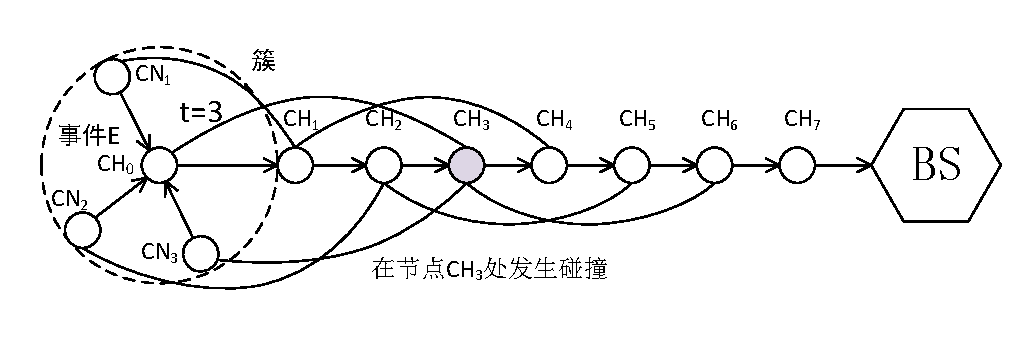
\includegraphics[width=5in]{IHAA4}
  \caption{动态步长多节点联合数据认证}
  \label{fig:IHAA4}
\end{figure}
\subsubsection{面向动态步长多节点联合数据认证的密钥分配}
%密钥分发,节点关系
在动态步长多节点联合数据认证中,我们也使用单向hash链来完成认证密钥的分配。不同于图~\ref{fig:IHAA3}中所示的密钥分配,在步长动态变化时,上下行相关节点组会发生碰撞,也就是不同的簇节点在同一个上下行相关节点组当中。如图~\ref{fig:IHAA4}中,节点$CH_0$和节点$CN_3$在同一个上下行相关节点组中,上行相关节点都是节点$CH_3$。

对于上下行相关节点的碰撞,我们通过对簇内节点添加虚拟的上下行顺序来解决。在如图~\ref{fig:IHAA4}的传输路径上,将4个簇节点的虚拟上下行关系设为$\{CN_3,CN_2,CN_1,CH_0\}$,也即步长为3时,节点$CH_0$是节点$CN_3$的上行相关节点。

\begin{figure}[htbp]
  \centering
  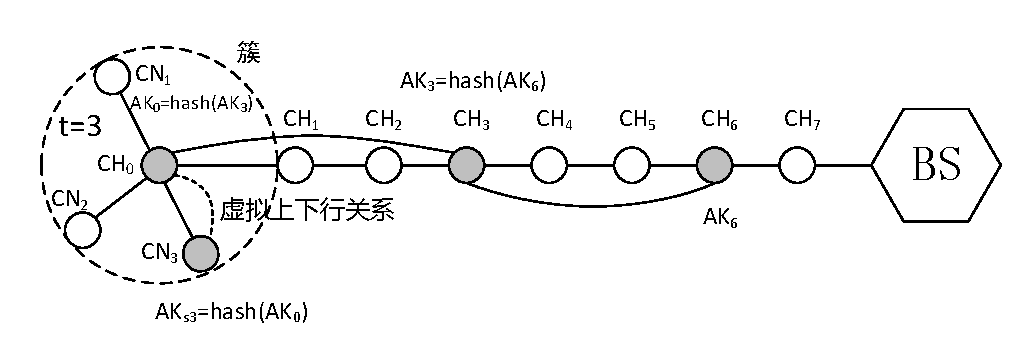
\includegraphics[width=5in]{IHAA5}
  \caption{面向动态步长多节点联合数据认证的密钥分配}
  \label{fig:IHAA5}
\end{figure}

如图~\ref{fig:IHAA5}所示,即为图~\ref{fig:IHAA4}所示的动态步长多节点联合数据认证情景的密钥传输示例。节点$CH_0$和节点$CN_3$都是簇节点,但是在同一个上下行相关节点组内,所以在节点$CH_0$和节点$CN_3$之间虚拟上下行相关关系,节点$CN_3$的密钥从节点$CH_0$的密钥计算而来,$AK_{s3}=H(AK_0)$。
\subsubsection{报文数据压缩传输}
使用单向hash链的密钥分配方案,给虚拟上下行相关节点分配了密钥以后,如图~\ref{fig:IHAA4}的动态步长多节点联合数据认证中,节点$CH_0$ 对簇节点数据进行整合之后的报文R可以表示为:
\begin{equation}\label{report3}
\begin{split}
  R=
  & E,C_i,h_0,XMAC(E),\{MAC(AK_{s1},E),MAC(AK_{s2},E),\\
  & MAC(AK_0,E)\oplus MAC(AK_{s3},E)\}
\end{split}
\end{equation}
其中$MAC(AK_0,E)\oplus MAC(AK_{s3},E)$为节点$CH_0$和节点$CN_3$的簇节点MAC使用XOR运算压缩后的结果。

我们用$p$表示步长,对于$h-h_0\leq p$的节点,在收到报文后,首先计算其下行相关节点的密钥。在图~\ref{fig:IHAA4}的示例中,节点$CH_3$ 收到报文R以后,首先计算下行相关节点的密钥$AK_0=H(AK_3)$。对事件E计算消息认证码$MAC(AK_0,E)$,并与报文R中第
$(h_0 - h_i)-((h_0 - h_i)/p)\ast p=3$个MAC进行比较,如果相同则用$MAC(AK_3,E)$替换之。如果不同则计算间隔一跳的下行相关节点的密钥$AK_{s3}=H(AK_0)$,对事件E计算消息认证码$MAC(AK_{s3},E)$,并与$MAC(AK_0,E)$进行XOR运算,
$MAC(AK_0,E)\oplus MAC(AK_{s3},E)$与报文R中第3个MAC进行比较,如果相同则用$MAC(AK_3,E)$替换之。
如果都不同,则表示是错误数据报文,但是不同于前面提出的方案,我们不将其直接丢弃,而是将$XMAC(E)$置为全0。
对于$h-h_0> p$的节点,同前述方案一样,只进行一次MAC验证。
在经过路径节点的验证后,节点将报文继续转发给上行节点。

\subsubsection{动态步长调整机制}
在BS收到报文以后,会对报文中的$XMAC(E)$进行验证。如果$XMAC(E)$为全0,则说明有错误数据报文在路径中被检测出来,这样说明传输路径的安全水平较低,则BS提高路径的传输步长$p$,这样能提升检测出错误数据报文的概率。如果BS连续收到若干个正常,达到一个阈值以后,我们认为路径是安全的,则BS降低路径的传输步长$p$,减小报文的大小,节约节点的传输能量。
\subsection{安全性能分析}


在BS收到报文以后,会对报文中的$XMAC(E)$进行验证。如果$XMAC(E)$为全0,则说明有错误数据报文在路径中被检测出来,这样说明传输路径的安全水平较低,则BS提高路径的传输步长$p$,这样能提升检测出错误数据报文的概率。如果BS连续收到若干个正常,达到一个阈值以后,我们认为路径是安全的,则BS降低路径的传输步长$p$,减小报文的大小,节约节点的传输能量。





\section{本章小结}
本章针对多节点联合数据认证机制中,节点失效或者受攻击对路径中的节点相关关系的影响,我们提出了多路径抗节点失效的机制,设计实现了相关算法。为了优化多节点联合数据认证的通信开销,我们设计实现了动态步长多节点联合数据认证机制。对两个优化方案,都进行了相关安全性能的分析。



